\vspace{-0.3cm}
\section{SOCIAL SIMILARITY}
Given the training social images with both visual features and social factors, our aim is to learn a distance function of visual features, which is consistent to the social similarity.  Therefore, we first need to explore how to evaluate social similarity of images according to their social behavioral information.
\vspace{-0.2cm}
\subsection{Image Presentation}
In this paper, we aim at embedding social behavioral information into visual space. Thus it is very important to present the complex and unstructured social behavioral information in a structured feature space. Here we call each dimension of social behavioral information as a social factor. Similar to the ``Bag of Visual Words" model in visual descriptor presentation, each social factor is presented in a ``Bag of social entity" way. For example, in Flickr, the typical social factors we can obtain include user favoring, group sharing, and user tagging, etc.  Thus an image can be presented by a set of users who favor it, groups that share it and tags that belong to it, which are defined as social entities. Therefore, a social image can be presented in visual and social dimensions, i.e., $\mathcal{I}_i = \{\mathnormal{x}_i, \mathcal{S}_i\}$, where $\mathnormal{x}_i$ is the vector of visual features ,and $\mathcal{S}_i=\cup_{k=1}^m \mathcal{V}_i^k$ is a set that includes $m$ social factors. $\mathcal{V}_i^k$ is the $k^{th}$ social factor of image $\mathcal{I}_i$. Each social factor $\mathcal{V}_i^k$ can be represented as a bag of social entities.   To make our formulation more general, we use the symbol $V_i$ to represent a social factor,  and $v_i$ to denote a social entity. For example,  we can use $\mathcal{V}^1$ to denote the social factor of user favoring. Therefore, $\mathcal{V}_i^1 = \{v_{t_1}, \cdots, v_{t_n}\}$ denotes that there are $n$ users $v_{t_1}, \cdots, v_{t_n}$ that favor the image $\mathcal{I}_i$.

Given the training social images with both visual features and social factors, our aim is to learn a distance function $d(x_i, x_j)$ of visual features, which is consistent to the social similarity $sim_{social}(\mathcal{I}_i, \mathcal{I}_j)$.  In this section, we will show some analysis of social factors and introduce how to evaluate the social similarity in our approach.
\vspace{-0.2cm}\subsection{Preliminary Study of Social Factors}
%���ݷ���
In our problem, the first question is whether the social similarity, i.e., the similarity of social factors is helpful in understanding image similarity in user behavioral aspect. To demonstrate this, we collect a social image dataset from Flickr, which includes 19,888 images, 6,843 users, 1,490 groups and 17,922 tags. For each user, we hope that all images that he/she  favors should have low variance in feature space because they confirm to his/her interests. Therefore, for the images that are favored by a given user, we extract visual features and social features and calculate the variance. Here the visual features are presented in a ``Bag of Visual Word" model. For each social factor, social feature is presented as the distribution vector of social entities. For example, if user $j$ favors image $i$, the $j^{th}$ element of the image $i$'s user feature is $1$, otherwise it is $0$. So are the group feature and tag feature. Each feature vector is normalized to make the 2-norm to be 1 for scale unification. For each user and group, the variances of the images in different feature spaces are illustrated in Figure \ref{preliminary}. From Figure \ref{preliminary}, we can observe that variance of visual feature is the largest among four features. Thus if we want to recommend images  to a user or a group, social similarity is more reliable than visual similarity. Among three social factors, we can find that the user favoring factor obtains the smallest variance. In other words, using others' favoring information to recommend images will obtain a good performance. This result is consistent with the idea of Collaborative Filtering (CF). In addition, we can see that most of the variance values are relatively large. It indicates that the images favored by a user or a group are usually very diverse in feature space.
\begin{figure}
\centering
\subfigure[]{
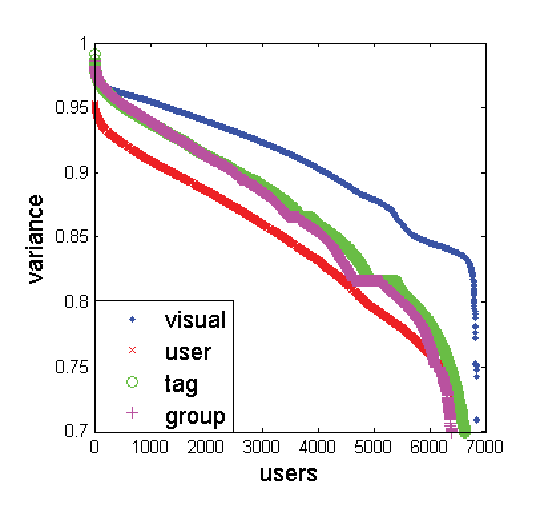
\epsfig{file=preliminary_1.eps, width=1.5in}
}
\subfigure[]{
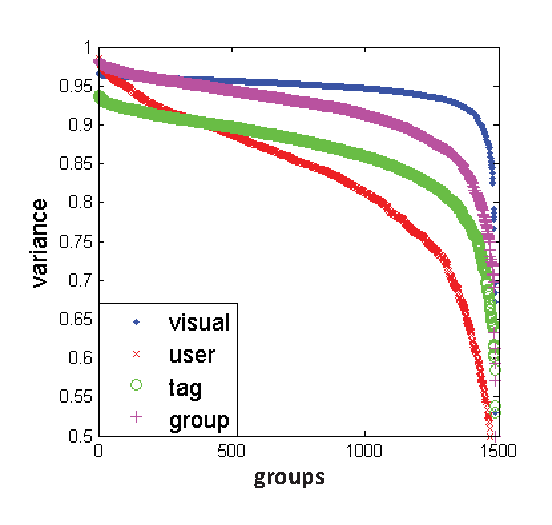
\epsfig{file=preliminary_2.eps, width=1.5in}}
\caption{The variance of the visual features and social factors of the images that are favored by each (a) user (b) group. The results are sorted in a descending order.}
\label{preliminary}\vspace{-0.3cm}
\end{figure}
\vspace{-0.2cm}\subsection{Reliability of Social Entities}
In social media, the user behavior information is usually noisy and uncertain. Thus not all social entities are equally reliable in evaluating social similarity. For example, images in the group named ``iphone club" should be similar but images in the groups named ``beautiful world" may be very diverse. In this case, the former group is more reliable than the latter one in similarity evaluation. Therefore, it is important to evaluate the reliability of social entities.

Take users as an example, if an image is favored by two users, we can assume that the interests of these two users are partially similar. Based on this assumption, we can build a similarity graph based on user interests. The nodes are users and the weight of an edge denotes the similarity of the users. We use $Im(v_i)$ to denote the images that are favored by user $v_i$, i.e.,
 \vspace{-0.1cm} \begin{equation} \vspace{-0.1cm}
 Im(v_i) = \{\mathcal{I}_t|v_i \in \mathcal{V}_t\}.
 \end{equation}
 In this equation, $\mathcal{V}_t$ denotes the all entities that belongs to image $\mathcal{I}_t$. Then, the similarity of the social entities can be defined as the Jaccard distance of the images:
 \vspace{-0.1cm} \begin{equation} \vspace{-0.1cm}
 sim(v_i, v_j) = \frac{|Im(v_i) \cap Im(v_j)|}{|Im(v_i)\cup Im(v_j)|}.
 \label{sim1}
 \end{equation}
 Based on the  similarity graph, we utilize spectral clustering method to divide users into $c$ clusters. For a given entity $v_i$, if all of its neighbors belong to the same cluster with $v_i$, we can think $v_i$ is a reliable social entity. The images belongs to user $v_i$ should have high probability to be similar. Thus, the reliability score of $v_i$  is defined as follows,
\vspace{-0.1cm} \begin{equation} \vspace{-0.1cm}
r(v_i) = \frac{1}{|c(v_i)\cup_{v_j \in N(v_i)} c(v_j)|},
\label{sp}
\end{equation}
where $N(v_i)$ is the set of neighbor nodes of $v_i$; $c(v_i)$ is the label of $v_i$'s cluster. If all of $v_i$'s neighbors  belong to the same cluster with it, the reliability score $r(v_i)$ is defined as $1$. On the contrary, if his neighbors cover all of $c$ clusters, $r(v_i)$ is defined as $1/c$.

This method is also suitable for the cases of using group or tag as social entity. For any entity $v_i$, the pair-wise similarity can be similarly calculated by Equation \ref{sim1} and the reliability score can be calculated by Equation \ref{sp}.
\vspace{-0.1cm}\subsection{Evaluation of Social Similarity}
We explore evaluating the social similarity of pair-wise images based on the reliability scores of the corresponding social entities. For two images $\mathcal{I}_i$ and $\mathcal{I}_j$, we analyze their similarity by their social factors $\mathcal{V}_i$ and $\mathcal{V}_j$. If $\mathcal{V}_i\cap \mathcal{V}_j$ is empty, i.e.,they share no common entities, we define the social similarity as 0. Otherwise, the social similarity is determined by the overlap of the entities and their reliability. Taking users as an example, intuitively, when the users have the same reliability, the images that are jointly favored by more users should be more similar. If the images are both favored by a fixed number of users, the images that are favored by more reliable users should have higher similarity. Based on the above two considerations, the social similarity of image in the social factor $\mathcal{V}_i$ and $\mathcal{V}_j$ is defined as follows,
\vspace{-0.1cm} \begin{equation} \vspace{-0.1cm}
sim(\mathcal{V}_i, \mathcal{V}_j) \!=\! \left\{\!\! \begin{array}{ll}
0, \!\!\!& \mathcal{V}_i \cap \mathcal{V}_j = \phi\\
\frac{\sum_{v_t\in \mathcal{V}_i \cap \mathcal{V}_j} r(v_t)}{\sum_{v_t \in \mathcal{V}_i \cup \mathcal{V}_j} r(v_t)}, \!\!\!& \textrm{otherwise}
\end{array}\right.
\label{sim2}
\end{equation}
where $r(v_t)$ is the reliability score defined in Equation \ref{sp}. In Equation \ref{sim2}, the similarity is defined as the weighted Jaccard similarity of $\mathcal{V}_i$ and $\mathcal{V}_j$. Obviously, this definition of similarity satisfies the previous heuristics. For a social image has multiple social factors, the final similarity of images $\mathcal{I}_i$ and $\mathcal{I}_j$ is defined as the average of all the social factors' similarity:
\vspace{-0.1cm} \begin{equation} \vspace{-0.1cm}
sim_{social}(\mathcal{I}_i, \mathcal{I}_j) = \frac{1}{m} \sum_{k=1}^m sim(\mathcal{V}^k_i, \mathcal{V}^k_j).
\label{social_sim}
\end{equation}
In this equation, we use average because different social factors reflect different aspects of image similarity. The final social similarity values range from 0 to 1. When the similarity is close to 1, the images are judged very similar in social dimension. On the other hand, when the similarity is near to 0, we are not very certain that the images are very dissimilar because similar images may also have no social relation. This problem can be solved by multiple sampling. Because of the diversity of the images, for a given image, if we randomly select many socially dissimilar images, the vast majority of them will be truly dissimilar to it.
